% Created 2023-12-21 Do 18:45
% Intended LaTeX compiler: pdflatex
\documentclass[11pt]{article}
\usepackage[utf8]{inputenc}
\usepackage[T1]{fontenc}
\usepackage{graphicx}
\usepackage{longtable}
\usepackage{wrapfig}
\usepackage{rotating}
\usepackage[normalem]{ulem}
\usepackage{amsmath}
\usepackage{amssymb}
\usepackage{capt-of}
\usepackage{hyperref}
\usepackage[a5paper, total={128mm, 190mm}]{geometry}
\usepackage{multicol}
\setlength{\parindent}{0pt}
\setlength{\itemsep}{0.mm}
\usepackage{enumitem}
\setlist[itemize]{noitemsep}
\usepackage[table]{xcolor}
\usepackage[type={CC},modifier={by-sa}, version={4.0}, imagewidth=5em]{doclicense}
\renewcommand{\familydefault}{\sfdefault}
\makeatletter
\usepackage[explicit]{titlesec}
\titleformat{name=\section,numbered}[block]{\normalfont\Large\bfseries}{}{0em}{\colorbox{black!100}{ {\color{white}\thesection\quad #1} }}
\titleformat{name=\subsection}{\normalfont\large\bfseries}{}{0em}{\colorbox{black!66}{ {\color{white}\thesubsection\quad #1} }}
\titleformat{name=\subsubsection}{\normalfont\normalsize\bfseries}{}{0em}{\colorbox{black!33}{ {\color{black}\thesubsubsection\quad #1} }}
\makeatother
\renewcommand\maketitle{
\begin{titlepage}
\centering
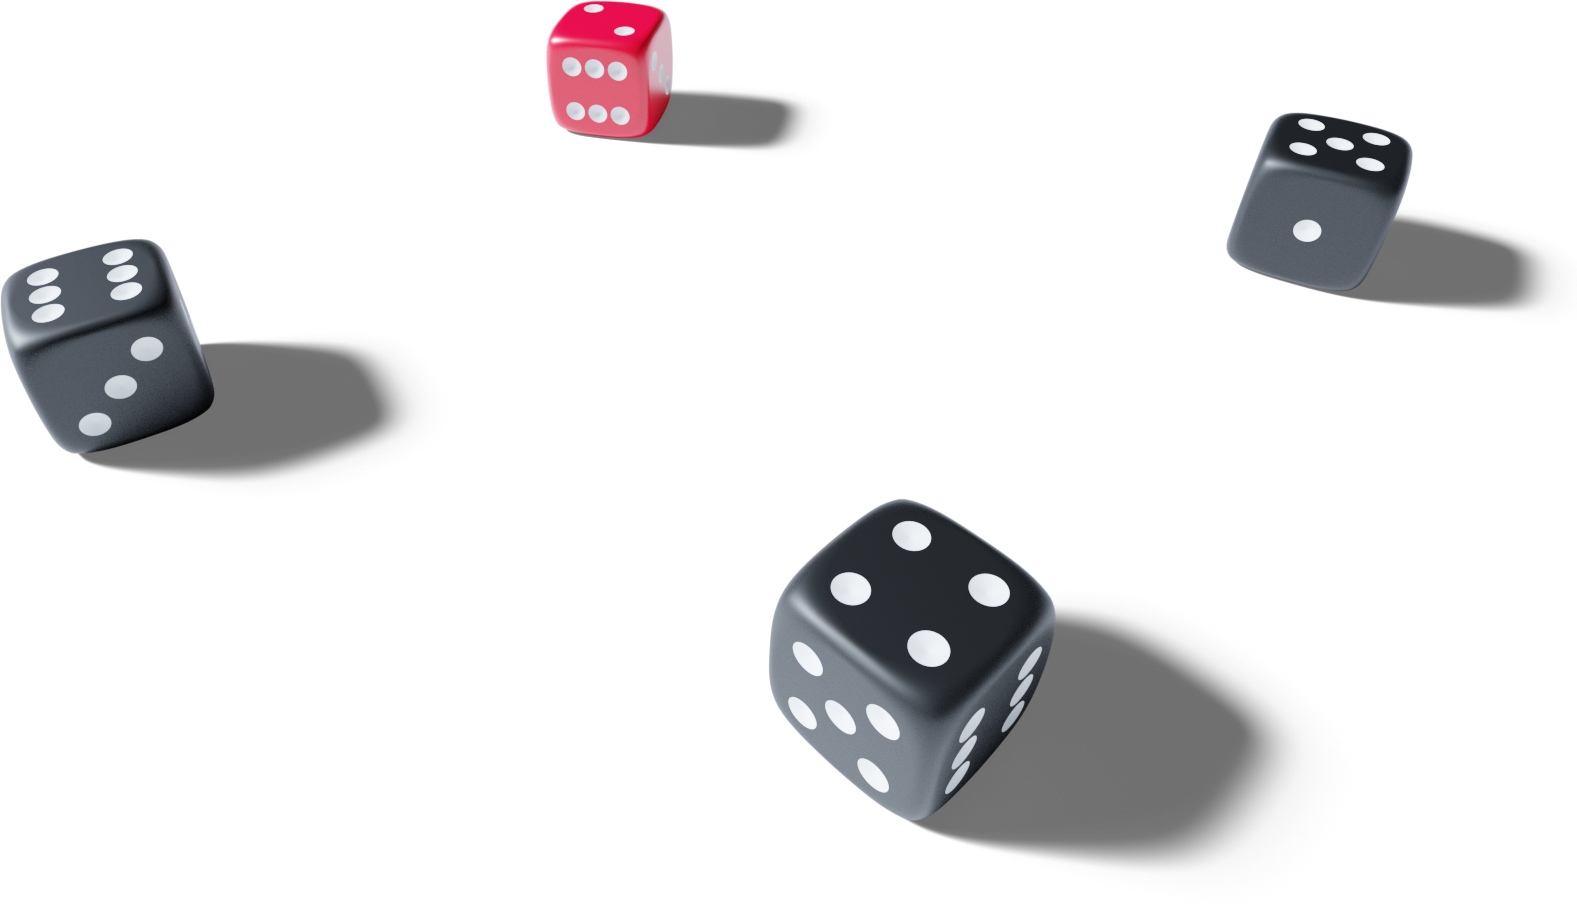
\includegraphics[width=0.8\textwidth]{dice_cut.png}
\topskip250pt\vspace{5cm}
\fboxsep2em\colorbox{black!100}{
{\color{white}\bfseries\fontsize{24pt}{29pt}\selectfont \quad Primordial Waters\quad\par}
}
\vfill
a game by\par
\textsc{Lukas Zumvorde}

\vfill

% Bottom of the page
{\large \today\par}
\end{titlepage}}
\usepackage{xparse}
\usepackage{soul}
\setcounter{secnumdepth}{3}
\date{}
\title{Primordial Waters}
\hypersetup{
 pdfauthor={Lukas Zumvorde},
 pdftitle={Primordial Waters},
 pdfkeywords={},
 pdfsubject={},
 pdfcreator={Emacs 29.1 (Org mode 9.6.6)}, 
 pdflang={English}}
\begin{document}

\maketitle
\tableofcontents

{\rowcolors{1}{grey!20}{grey!10}


\section{Introduction}
\label{sec:org0b918a0}

Primordial waters is a generic, light, and abstract role playing rule set with a focus on keeping the game balanced while maintaining and even promoting creative story telling. It leans towards a cinematic play style.

\subsection{Goals}
\label{sec:org20e5481}

\paragraph*{Rules Light}
\label{sec:org450303a}

The intend is for the rules to be as small as possible given the other goals. It should be easy to get into the game and easy to check the rules if you are not sure how a situation should be handled.

\paragraph*{Easy to Modify}
\label{sec:orgc8cd49d}

It should be easy to create useful house rules to make the game fit your campaign.

\paragraph*{World Agnostic}
\label{sec:orgaf0d97d}

The game should work with any game world or type of story reasonably well.

\paragraph*{Scalable characters}
\label{sec:org0c32246}

It should be possible to play both super-humans and commoners. It should also be possible to use the same rules to display rats vs humans or humans vs. giant spaceships. Imagine a giant space battle taking place outside and the group of players running around as mere humans performing acts of sabotage to tip the battle in their sides favor. 

\paragraph*{No action economy}
\label{sec:org99447ff}

It should be possible to do multiple things simultaneously in a round. It should be a trade off. This adds a new dimension of interesting decision making to the game.

\paragraph*{Constistent propability distribution}
\label{sec:org72e51cb}

No matter how powerful a character is, The probability distribution for his die rolls should be consistent and allow for interesting scenarios to occur. It should still feel fair.

\paragraph*{Easy Preparation}
\label{sec:org687a885}

The game should allow GMs to prepare new characters and challenges easily and quickly. It should get out of his way, but still support him in keeping the games balance.

\paragraph*{Creative Character Build}
\label{sec:org99f1bbf}

Players should be able to create nearly any character they like. It should also be possible to change the character at any point in the campaign to reflect the characters development. In this the rules should invite creativity and just ensure the games balance.

\paragraph*{Support interesting storys}
\label{sec:orgc82ce94}

The rules should support the creation of interesting and consistent storys by providing anker points for unexpected results.

\paragraph*{Keep Game Balance}
\label{sec:orgb6ac935}

In order for all to enjoy the game it must feel fair. Player characters need to feel similarly useful and encounters with NPCs or challenges must feel beatable but challenging.

\paragraph*{Rules Out of your way}
\label{sec:orga5a0d92}

The rules should be there to help you keep the games balance, but they should not prevent you from creating the story you want to create.

\paragraph*{No extensive Bookkeeping}
\label{sec:orgeb736dd}

The game should be playable without extensive bookkeeping. IT should not be necessary to fill out a multiple pages long character sheet. During the game it should not be necessary to calculate or evaluate many values.

\subsection{Inspirations}
\label{sec:org38b5328}

This game did not come from nothing. Many other games had an impact on its creation. Some of the most impact full ones are the following.

This games systems for aspects and movement were heavily inspired from the Fate Core system.
Karma was originally inspired by Fate Cores Fate Points, but EZD6 had the better name for the concept.
The distribution of attributes into categories was inspired by the AERA RPG.
The fate die to create unexpected events was inspired by the One Page Solo RPG Engine.
The optional rule "Only Players Roll" is taken from the Cypher System.

\subsection{How to use the game}
\label{sec:org6c6f0e6}

First rule of Gaming: Have fun. If the rules hinder you from having fun then screw the rules.

Second rule of Gaming: When in doubt use common sense. The rules will never be perfect. If something is illogical when using the rules or if no rules exists for the situation then feel free to find your own ruling. 

Third rule of Gaming: Use the aspects value as a guideline and be creative with what it could mean. Does a flame wall having a value of 4 mean that it has a difficulty of 4 to jump over it or does it attack anyone jumping over with 4 dice? Do what fits your story. 


\subsection{Conventions}
\label{sec:org4ab0713}

In the book we use the following shorthands.

A \(N d_0 X\) means rolling dice with 0 to X as possible results N times and adding the results. Since there are very few dice that that have a 0 as a possible result you can use other methods to get the result. I suggest to draw a playing card.

To use Playing cards instead of dice you can do the following. Take a standard 54 card deck of playing cards. Remove the 2 Jokers from it. Shuffle and pick a card. If it is a number then take the number as a result. Aces count as 1. Jacks count as 11, Kings count as 12. Queens count as 0 since Q looks most like a 0.

The rules often mention a dice pool. This pool is hypothetical. It means if you always used a number of  \(d_0 2\) to perform any check this would be your dice pool. A \(d_0 2\) has an average result of \(1\). Therefore the dice in the dice pool is always exactly the average result of a check. This does not mean you have to roll your checks in that way.


\subsection{What dice to roll}
\label{sec:org6f8610d}
\begin{itemize}
\item \(1 d_0 2\) is worth exactly 1 dice from the pool (this is the default)
\item \(1 d_0 N\) is worth \(\frac{N}{2}\) dice from the pool
\item \(1 d N\) is worth \(\frac{N+1}{2}\) dice from the pool
\item Take the average: \(N\) constant points is worth \(N\) dice from the pool
\item Any dice multiplied by a factor \(F\) is worth the price of a single dice multiplied by this factor \(F\)
\end{itemize}

The default is to use \(F \times 3 d_0 2 + c\). This means that the factor \(F\) is the dice pool divided by 3 with c being the remainder. The players are free to use any other combination of dice they like as long as they don't exceed the dice pool.

\newpage
\section{Rules}
\label{sec:orgdee138c}

\subsection{Attributes}
\label{sec:org971eef4}
Attributes describe a characters potential. The higher the value the greater things a character can achieve. There are the following 8 Attributes belonging to the 4 categories.

\begin{center}
\begin{tabular}{lll}
\textbf{Category} & \textbf{Attribute} & \textbf{Description}\\[0pt]
\hline
Physical & Strength & strength and hardiness\\[0pt]
 & Dexterity & agility, speed, precision\\[0pt]
\hline
Mental & Will & perseverance, attention\\[0pt]
 & Intellect & intelligence, knowledge\\[0pt]
\hline
Social & Empathy & understanding people\\[0pt]
 & Charisma & interacting with people\\[0pt]
\hline
Resources & Gear & Gear you have prepared\\[0pt]
 & Finances & Money and investments\\[0pt]
\end{tabular}
\end{center}

The attributes value is the basis for the dice pool one has available for \hyperref[sec:orgdb9101c]{checks}. 

\subsection{Aspects}
\label{sec:org0141223}
Aspects are a combination of a descriptors and a value. When invoked the aspects value is added or subtracted from the number of dice rolled for \hyperref[sec:orgdb9101c]{checks}. An aspect is always bound to something. Be it a player, a NPC, an object or even a zone. Be creative with aspects. Try to bind their effects to the value and they should stay balanced enough.

\paragraph*{Creating an Aspect}
\label{sec:org4dc7e3f}

An aspect can be created at any time by the GM. It can also be created by any player, NPC or even object. To create an aspect all but the GM need to make a check. The aspect points (AP) from this check can be used to create an aspect. Increasing an aspects value by 1 costs 1 point. The description of the aspect can be decided freely. 

\begin{quote}
Arthur the mage wants to enflame the gras around him to channel the enemies into a one on one battle with his Companions. The GM likes this idea and creates the aspect "Dry Grass 1" that Arthur can use. Arthur decides to cast his spell, succeeds with 3 AP, and creates the aspect "Wall of Fire 3". Now any enemy has to either go around the wall or get burned. If an enemy tires to jump through, they have to roll on it against the Fires 3 dice. If the fire succeeds they get burned.
\end{quote}

\paragraph*{Using Aspects}
\label{sec:orgde0d765}

Whenever it makes narrative sense an aspect can be used. When used an aspect adds its value to the number of points that can be used for a check. It is also possible to call out an aspect to be used to hinder a check. Then the value is subtracted from the points instead. An aspect can both be used for actions and reactions but never at the same time. If you use aspects in a contest make sure that aspects are not used more than once per round by a character or their points are distributed over different actions.

\paragraph*{Area Aspects}
\label{sec:orgbe93062}

An aspect can affect a zone. This means it can be invoked for all in the zone. To create such an aspect costs double the points. Exceptions may be made by the GM. 

\paragraph*{Multiple Targets}
\label{sec:org3046abd}

If an aspect impacts multiple targets it costs double. Exceptions may be made by the GM.

\paragraph*{Duration of Aspects}
\label{sec:orgd4e441c}

An aspect can be over within a round or it can last longer. Normally aspects last at least a scene long. If your aspect should last longer it should cost double. If it should only last for a round the costs half. Exceptions may be made by the GM. In general it can be said, that an aspect lasts as long as it makes sense.

\paragraph*{Acting Aspects}
\label{sec:orgd6a0157}

Sometimes an aspect should perform actions on its own. Each round they can act like any other player or NPC. They use their value for their actions.

\begin{quote}
Poison Cloud 2: Each round it tries to use 2 dice to poison any inside. Since it impacts a zone it can do this for everyone inside the zone every round.
\end{quote}

\paragraph*{Resistant Aspects}
\label{sec:orgb879210}

An aspect can have resistance to being removed. The resistance is subtracted from any attempt to removing this aspect. For each point of resistance costs 1. The effective resistance can never be more than the aspects value. Be creative when invoking a resistant aspect. For example armor could be implemented as an aspect with resistance.

\begin{quote}
A heavy door blocks the way. The GM creates the aspect "Fortified Door 5[2]". This means the aspect has a value of 5 with a resistance of 2. The players try to break through with pure strength. On their first try they get 4 AP. 2 get absorbed by the doors resistance and the rest weakens the door. The door s aspect is now "Fortified Door 3[2]". On their second try the players get 6 AP and break throgh.
If the players had decided to pick the lock the GM may had ignored the restistance value.
\end{quote}


\paragraph*{Character Aspects}
\label{sec:orgff89a2b}

Aspects can also be bound to a character and be bought with CP. If an aspect is mostly negative in nature it may give you points instead. Character aspects can be invoked by the GM to make the character do something. The player can always decline this, but this costs one karma.

\paragraph*{Damage}
\label{sec:orga70536f}

Aspects are also used to represent damage a character or object has taken. If a character is unable to act in a scene because too many aspects hinder him, it is a good idea to narrate them out of the scene. It is also a good time to create a fitting negative character aspect representing this loss (like "lost an arm" or "fear of water" or "hateful of orcs").

\subsection{Checks}
\label{sec:orgdb9101c}
Checks are rolled when the outcome of an action is not certain. Each check is bound to an \hyperref[sec:org971eef4]{attribute}.

Add the points in the relevant attribute and all applicable aspects together. This is your dice pool. Use the rules in \hyperref[sec:org6f8610d]{What dice to roll} to determine what dice to roll. You get the result of the roll in aspect points (AP).

If the aspect points are zero or negative the check fails.

\paragraph*{Difficulty}
\label{sec:org5136bdf}
The checks difficulty is the sum of all aspects that are to be overcome or created.


\paragraph*{Collaborative checks}
\label{sec:org53b03dc}
Everyone rolls individually and then sum together all AP.

\paragraph*{Risky checks}
\label{sec:org5ba67b3}
If a check is risky the character might incur something bad if the check fails. If the check fails a negative aspect is created worth the difficulty in points. The minimum is 1. You can not take the average on a risky check.

\paragraph*{Taking Time}
\label{sec:org792b732}
Sometimes a check is to difficult to achieve something within 1 check. Then it may be possible to do multiple checks over a longer time to accumulate the points needed. However, you must decide beforehand how many checks you want to take. The AP of all checks are accumulated after considering the difficulty. The GM has a veto right.

\paragraph*{Unexpected Results}
\label{sec:org42a116a}
You roll an additional d6, called the fate die. On a 1 you add a "but .." and create an additional aspect worth the factor F in points that counteracts the result somewhat. On a 6 you add a "and .." and create an additional aspect worth the factor F in points that enhances the result somewhat. The extra die can also be rerolled with a fate point or advantage on the check.

\begin{quote}
"Success and" during a fight against a goblin. You decapitate the goblin in an intimidating display, Not only does the goblin die but the display also weakens the goblins resolve. Likely they will try to flee after seeing this.
Aspect: Intimidating display 2.
\end{quote}

\begin{quote}
"Success but" during a fight against a goblin. You kill the goblin but are now covered in his blood, This has no effect on the fight itself but it may hinder any piece negotiation or help you when intimidating the remaining enemies.
Aspect: Covered in Blood 2.
\end{quote}

\subsection{Contest}
\label{sec:org1ed98bf}
The prototypical contest is combat, but the same rules can be used any scenario where multiple parties act in opposition to each other. Be it a diplomatic debate or the hostile takeover of a company. 

A contest is divided into rounds. Each participant in the contest can make one or more actions each round. When it is a participants turn or on any later point in the round they can perform an action.

\paragraph*{Actions}
\label{sec:org29c050d}
An action is a check that tries to create an aspect. Any kind of aspect can be created, based on what fits the scene. You can try to gain an advantageous position, or start a big fire.

If in combat the aspect that is created it is by default \texttt{stress}. If a character has more \texttt{stress} than he has points in an attribute, then  he can not use this attribute any more. Once the scene ends the stress is converted to one or multiple negative aspects like wounds or exhaustion. 

\paragraph*{Reactions}
\label{sec:org8e9ae5e}
Whenever someone takes an action and has rolled his dice anyone else can immediately try to perform a reaction to prevent it. A reaction does not by its nature create an aspect. If you announce this before the action is rolled you can take the average on a reaction. You have to announce the number of dice invested. The points from the reaction are then subtracted from the points of the action to lessen its effect.

\paragraph*{Turn Order}
\label{sec:org30f9590}
The participants take turn from the one with the highest relevant attribute (+ aspects) to the lowest. On your turn you don't have to act. You can act at any point after you turn in the turn order. Even multiple times. 

\paragraph*{Multiple (re)actions}
\label{sec:org34287f8}
Each round you can take multiple actions and reactions. The total number of points gained from the attributes is the largest attribute value of the checks. From each attribute you can use at most its value in points in total. Each Aspect can only be used once or their AP (attribute points) have to be distributed to the (re)actions.

\paragraph*{Acting together}
\label{sec:org0a48905}
When acting together all values are combined and a single combined check is made or alternatively only the AP are combined. To act together all have to act at the same time in the turn order, so effectively at the earliest when the slowest has his turn.

\subsection{Karma}
\label{sec:org3b80861}
Each player can have up to 3 karma. They can be used at any point in time to change a single die roll (not just your own) to any specific value or to add an interesting aspect to a scene (GM has veto rights). Karma can be recovered by a characters aspect being used against them or as a reward for good role play (anything that brings joy to all players and the GM). Players should start a session with 2 karma.


\subsection{Traits}
\label{sec:org2c9a819}
Traits are distinguishing things about the character that allow him to break a rule of the world or the game in some way. For example with the Trait Night Vision you can just see in the dark. No rolls required. Some traits (like all magic) should come with a risk, meaning all checks that can only be made with this trait are risky checks. They can be bought for character points, this is possible both at character creation and later in the game.

See the chapter \hyperref[sec:orga817fd6]{List of Traits} for examples.

\subsection{Character Creation}
\label{sec:org0023269}
Distribute 100 CP on your Attributes, Aspects and Traits.

Use the rules under equipment to limit your starting gear.

Character Advancement:
You may reward your players with CP (character points) for reaching milestones in the story or simply surviving the session.

\begin{itemize}
\item An attribute point costs 4 CP.
\item An Aspect point typically costs 4 CP but can vary based on how specific they are.
\item A Trait typically costs 10 CP but can vary widely. Negative traits can even have a negative price.
\end{itemize}

A typical player character will have:
\begin{itemize}
\item all attributes with value 2 on average
\item 3 aspects with value 2
\item 1 trait
\end{itemize}

\subsection{Movement and Range}
\label{sec:orgcfd2a33}
Sometimes it is useful to draw maps and define distances. In a contest split the area into roughly 3-5 zones. A character can move from one zone to another each round. If one can act at a range like for example when shooting a bow one can act 1-2 zones far. During the round a character is moving he can be considered to be in both zones at once.

\subsection{Items and Equipment}
\label{sec:org115c7a1}
Items have a description and a resource value (RV). The RV is an abstraction for the items price or usefulness. 
Items may have an aspect associated with them. If you want items to have any specific effects you may add aspects. At any time the GM can choose to give an item an aspect. Normally it will have the resource value of the item in AP. You don't have to write down the obvious aspects an item has. For example you dont need to specify that the sword is good for slicing stuff.

A few examples can be found in the section \hyperref[sec:orge59c6d9]{List of Items}.

\begin{center}
\begin{tabular}{c|l|l}
\textbf{RV} & \textbf{Description} & \textbf{Example}\\[0pt]
\hline
0 & Free & a club\\[0pt]
1 & Cheap & simple clothes, basic tools\\[0pt]
2 & Affordable & regular car, apartment\\[0pt]
3 & Costly & regular house\\[0pt]
4 & Expensive & sports car\\[0pt]
5 & Very Expensive & small airplane\\[0pt]
6 & Luxurious & private jet\\[0pt]
\end{tabular}
\end{center}

\paragraph*{Armor / Damage Reduction}
\label{sec:org0c88bc4}
There is no Armor but some aspects can act as such. If an aspect can be used in a defensive (re)action, this effectively reduces the amount of AP of the attack. Thus they act like armor. Think of armor items as having the protective aspect on them. If an aspect can be used is up to the GM. So he can decide that the very expensive ballgown can not be used to defend against a bullet.

\paragraph*{Equipment}
\label{sec:orgb26f54e}
Characters can have gear with a value of up to the attribute Gear in RV on them. They must be able to carry all that gear on them or if it is part of their household it must fit in their normally furnished home. Apply reason as necessary.

When out adventuring characters have all the gear that they have written down. Additionally they can be allowed to make a Gear check against the RV of what they would like to have in the moment to see if they do. The check is risky and if they fail they get the difference in damage to their Gear attribute until the end of the mission.

\paragraph*{Buying}
\label{sec:org255a2de}
Characters can buy new items with a Finances check. The check is risky. The bought item can be treated like an aspect that is created with this check. The GM does not have to let you retry on a fail. If you use items with aspects to do this like the "Treasure" you found during your last adventure you may lose them if you succeed on the check.

\paragraph*{Crafting}
\label{sec:orgd1cf44b}
Characters can also build their own items. For that they need the appropriate tools and resources. The resources may be bought and have a RV of the item to be build minus 1. To build the item the character needs to make a check with the items RV as difficulty. If that fails the resources might be lost, depending on what they are.

\paragraph*{Gathering}
\label{sec:orge0e513a}
Resources can be gathered with a check and their RV as difficulty.

\paragraph*{Creating}
\label{sec:org4bcdae0}
To create an item first give it a short description. Second you determine its value if applicable. Add aspects if applicable. 

\paragraph*{Bribing}
\label{sec:org09a9945}
To Bribe someone you need to give them more than they can normally comfortably afford. This means you need more than their finances value in RV to bribe them.

\section{Optional Rules}
\label{sec:org345f5a9}
\subsection{Magic}
\label{sec:org4baea31}

Magic gives a huge narrative flexibility to explain aspects. To balance this out any checks made using magic should be considered risky. This means the value of the created aspects has to be defined beforehand. This is taken as the difficulty of the check. If the check fails the magician creates an unwanted likely negative aspect at the value of the difficulty. If he succeeds the created aspect has exactly the predefined value. Depending on the setting a trait might be necessary to cast magic or even a specific kind of magic.

\subsection{Less precise Attributes}
\label{sec:org9404024}

Instead of using the Attributes as listed you can use only the Categories. Learning a level in one of the categories costs double of what a level in an attribute would cost.

\subsection{No Abstraction for Wealth}
\label{sec:org5669a7d}

To remove the resources category from the attributes just raise the price of learning a level of the other attributes by 33\%. The costs for goods and services
depend on the campaign setting.

\subsection{Retroactive Actions}
\label{sec:orgd186e58}

The GM may allow players retroactively having performed some action. For example having placed a trap beforehand. To balance this any check on such an action should be a risky check.

\subsection{Quicker Battles}
\label{sec:orgae3023d}

Instead of differentiating between attacking and blocking you can speed up combat by handling it all as generic combat. If someone initiates combat with his action, others may react with combat in return. Whoever wins the contest makes the difference as a damaging aspect.

\subsection{Stress in Contests}
\label{sec:orgaa8fc31}

To speed up and simplify contests you can always create an abstract Aspect called "Stress". Stress does not hinder you in a contest but once it reaches the same value as your attribute you lose the contest. After combat stress converts into an appropriate aspect of equal size.

\subsection{Only Players Roll}
\label{sec:org955b59b}
If you like you can generally let only players roll the dice. Everyone else will take the average result. This means that in combat only players will roll to hit or roll to block.

\newpage
\section{Lists}
\label{sec:org3ec4cdc}
None of the following lists is exhaustive. They should be taken as examples. You are invited to design your own with your group.

\subsection{List of Traits}
\label{sec:orga817fd6}
\begin{quote}
\textbf{Friend of Nature} (7): You can talk to the forces of nature and have a chance to convince them to help you. This can be asking, a bird what he has seen, letting yourself be concealed by a bush or calling a wild bear to aid you in combat.
\end{quote}

\begin{quote}
\textbf{Illusionist} (7): You are adapt at creating illusions. The bigger and more complex they get the harder this is.
\end{quote}

\begin{quote}
\textbf{Speedster} (14): You have incredible speed. Others see only a blur when you sprint past them. This often gives you an advantage on dexterity checks and you always have at least 1 success in them. It takes you half the dice to move on a round.
\end{quote}

\begin{quote}
\textbf{Medium} (7): You can commune with ghosts and spirits. You have no control over them, but you can gain their attention.
\end{quote}

\begin{quote}
\textbf{Night-vision} (7): You can see in darkness as if it were light.
\end{quote}

\begin{quote}
\textbf{Sleepless} (7): You don't need sleep. This means you have a lot more time in a day, but you still need to rest from to much physical or mental exertion.
\end{quote}

\begin{quote}
\textbf{Flight} (16): You can fly. Be it with wings or otherwise. Your speed in flight is no different from your speed on land.
\end{quote}

\begin{quote}
\textbf{Tinkerer} (7): You can build wondrous mechanical marvels. From clocks up to steam powered automatons. 
\end{quote}

\begin{quote}
\textbf{Hacker} (7): You are not only proficient in computer science but you can even achieve movie worthy feats like stopping another car with only your laptop during a car chase. Tools not included.
\end{quote}

\begin{quote}
\textbf{Plot Armor} (3): Each scene you can disregards an aspect representing damage. 
\end{quote}

\begin{quote}
\textbf{Short Weapon Fighting} (1): You can not get disadvantage because your weapons are to short compared to your opponent.
\end{quote}

\begin{quote}
\textbf{Unarmed vs. Armed} (2): You can fight against armed opponents even when you have no weapon without disadvantage.
\end{quote}

\begin{quote}
\textbf{Alchemist} (7): You can brew potions, salves and other things which create wondrous effects.
\end{quote}

\begin{quote}
\textbf{Shape Shifter} (7): You can alter the physical form of either yourself or that of others.
\end{quote}

\begin{quote}
\textbf{Seeer} (7): You have to ability to see glimpses of future, past and present. Both at your current position and over great distances. 
\end{quote}

\begin{quote}
\textbf{Amphibious} (7): You can live both underwater and on land.
\end{quote}


\subsection{List of Items}
\label{sec:orge59c6d9}
\begin{quote}
\textbf{Sword} (2): Its a stabby piece of metal. Especially good at harming unarmored enemies. Not so great at slicing though armor. 
\end{quote}

\begin{quote}
\textbf{Mail shirt} (3): A metal fabric that protects your torso and arms from being cut or stabbed pretty well. However it helps little against blunt force trauma.
\end{quote}

\begin{quote}
\textbf{Club of the great Bear} (4): A mystical club made from the thigh bone of the great bear that terrorized the inokwa people. It still contains the strength of the mighty beast. When using this club you gain 1 in strength checks.
\end{quote}

\begin{quote}
\textbf{Knightly Armor} (4): A good example of heavy armor that protects from physical damage from most weapons.
\end{quote}

\begin{quote}
\textbf{Protective Amulet} (2): This amulet made from magically potent elder wood protects lightly (1 damage reduction) from mental damage coming from magic.
\end{quote}

\begin{quote}
\textbf{Pentagram Amulet} (2): This amulet was made to prevent possession and influence of otherworldly forces. Allows you to reroll 1 die against attacks against your mental state when coming from ghosts, magic, or similar forces.
\end{quote}

\begin{quote}
\textbf{Potion of Healing} (3): When being drunk it allows you to reduce the healing time of up to 3 physical damage from M to S
\end{quote}

\begin{quote}
\textbf{Shield} (2): Gives the reroll of 1 die when blocking with the shield.
\end{quote}

\begin{quote}
\textbf{Sword} (2): This stabby piece of steel typically makes class M damage. Its also good at slicing.
\end{quote}


\subsection{List of NPCs}
\label{sec:orgad6a9a8}
\begin{quote}
\textbf{Average Citizen} ( CP)
Ph:3, Me:3, So:3, Re:3
\end{quote}

\begin{quote}
\textbf{Goblin} ( CP)
Ph:2, Me:1, So:1, Re:1, Night Vision
\end{quote}

\begin{quote}
\textbf{Ratling} ( CP)
Ph:1, Me:1, So:1, Re:1, Strength in numbers 1
\end{quote}

\begin{quote}
\textbf{Wolf} ( CP)
Ph:3, Me:1, So:2, Re:0, Endless endurance 1
\end{quote}

\begin{quote}
\textbf{Guard} ( CP)
Ph:4, Me:3, So:3, Re:3
\end{quote}

\begin{quote}
\textbf{Dark Mage} ( CP)
Ph:3, Me:8, So:4, Re:6, Necromancer 3, Telepathic Link to undead servants
\end{quote}

\begin{quote}
\textbf{Ogre} ( CP)
S:16, D:8, W:6, I:2, E:2 ,C:2, G:1, F:1
\end{quote}

\begin{quote}
\textbf{Zombie} ( CP)
Ph:2, Me:1, So:1, Re:1, Infectious Bite
\end{quote}

\begin{quote}
\textbf{Bandit} ( CP)
Ph: 4, Me: 3, So: 2, Re: 2
\end{quote}

\begin{quote}
\textbf{Combat Drone} ( CP)
Ph: 3, Me: 1, So: 1, Re: 1, Shooting 4, Night-vision
\end{quote}

\begin{quote}
\textbf{Orc Veteran} ( CP)
Ph: 6, Me: 4, So: 3, Re: 3, Night Vision, Reckless and Bold 2
\end{quote}

\begin{quote}
\textbf{Orc Warrior} ( CP)
Ph: 4, Me: 2, So: 1, Re: 2, Night Vision, Reckless and Bold 1
\end{quote}

\begin{quote}
\textbf{Giant Spider} ( CP)
S: 2, D: 4, W:2, I:2, E:1, C:1, G:2, F:1, Night Vision, Spider Webs 2
\end{quote}


\newpage

\section{Advice}
\label{sec:orge249b49}
\subsection{Gameplay Notes}
\label{sec:org06a9e53}

Since aspects can appear, disappear and change frequently during play, it is good to write them down and show them to your players. For this i suggest to use post-it notes. This has the nice effect that you can give your players something physical that represents the advantages they created or can use.


\subsection{Character Creation}
\label{sec:org9ccd8d2}

When creating a character you should adhere to the following advice:
\begin{itemize}
\item No attribute above 6
\item No attribute below 2
\item Have 1 aspect describing what you want to be good at
\item Have 1 aspect describing how you make your living
\item Have 1 aspect describing what you like to do as a hubby
\item Forumlate your traits such that they can be interpreted as a vulnerability
\item Have at least 1 trait
\end{itemize}
Break these rules as you like.


\subsection{Encounter Design}
\label{sec:orga3fb67b}

To design a good challenge count the total of attributes and aspects the players could bring to the fight and match this with those of the opponents roughly 1:1.

\begin{itemize}
\item Sum the CP of your player characters
\item divide the sum by 100
\item multiply this with 3
\item The result is a good estimate for how hard a challenge should be.
\end{itemize}

A rough estimate can be to divide the sum of all your players CP by 100 and multiply this by 3.

Let your players become creative and create aspects to help them better their odds.

Try to give any noteworthy opponent an advantageous and a disadvantageous aspect.

\section{Game-play Examples}
\label{sec:orgccbec9b}
\subsection{Character Build: Alchemist}
\label{sec:org85d62ed}

\begin{quote}
\textbf{Anna the Alchemist}

Strength: 3
Dexterity: 3
Will: 4
Intelect: 6
Empathy: 4
Charisma: 3
Gear: 6
Finances: 6

Traits:
\begin{itemize}
\item Magical Alchemy
\end{itemize}

Aspects:
\begin{itemize}
\item Third daughter of an Aristocratic Family 2
\item Proud member of the Alchemists Guild of Mistwater 3
\item Hobby Horse Rider and Trainer 1
\end{itemize}
\end{quote}

\subsection{Character Build: Babarian}
\label{sec:org9d189fe}

\begin{quote}
\textbf{Bob the Barbarian}

Strength: 6
Dexterity: 5
Will: 4
Intelect: 3
Empathy: 2
Charisma: 4
Gear: 2
Finances: 2

Traits:
\begin{itemize}
\item Cold Resistance
\item Plot Armor: Can prevent getting a damaging aspect up to one time per scene.
\end{itemize}

Aspects:
\begin{itemize}
\item Member of the isolated Nomads of the eastern steppes 2
\item Best Fighter of his tribe and wrestling champion 3
\item Gambler 1
\end{itemize}
\end{quote}

\subsection{Character Build: Generic Citizen}
\label{sec:org6084e01}

\begin{quote}
Strength: 3
Dexterity: 3
Will: 3
Intellect: 3
Empathy: 3
Charisma: 3
Gear: 3
Finances: 3

Traits:
none

Aspects:
none
\end{quote}

\subsection{Character Build: Shapeshifting Durid}
\label{sec:org8e9a69a}

\begin{quote}
Strength: 4
Dexterity: 4
Will: 5
Intellect: 3
Empathy: 3
Charisma: 4
Gear: 3
Finances: 2

Traits:
\begin{itemize}
\item druidic magic
\item Magical alchemy
\item Shapeshifting
\item Seer
\end{itemize}

Aspects:
\begin{itemize}
\item Shapeshifting Druid 4
\item Protector of the Ancient Grove 3
\item Knowledgeable in the alchemy of the gifts of nature 2
\end{itemize}
\end{quote}

\subsection{Character Build: Space Pirate}
\label{sec:org8789291}

\begin{quote}
Strength: 3
Dexterity: 3
Will: 4
Intellect: 5
Empathy: 3
Charisma: 4
Gear: 3
Finances: 4

Traits:
\begin{itemize}
\item Bionic Eye with super zoom level and infrared vision. (7 CP)
\item Bionic Leg (1 CP)
\end{itemize}

Aspects:
\begin{itemize}
\item Has lift in space all his life 2
\item If the captain ordered it it has to be done 2
\item Space engineer 1
\item Gambler 2
\item Really good with the needle 1
\end{itemize}
\end{quote}

\subsection{Character Build:}
\label{sec:orgbdde041}

\subsection{Example: Ambushed by Goblins}
\label{sec:org60c03b4}

\textbf{GM} is the Game Master Mathew controlling the 3 goblins (P: 2, M; 1, S: 1, Life of Banditry 1)

\textbf{A} is the player Anna with her character Amy (P: 3,M: 6,S: 4, Proud member of the Alchemists Guild of Mistwater 3)

\textbf{B} is the player Ben with his character Boris (P: 6,M: 4,S: 3, Best Fighter of his tribe and wrestling champion 3, Member of the isolated Nomads of the eastern steppes 2)

\textbf{GM:} As you walk along the forest trail please roll for perception with your will.
\begin{itemize}
\item GM rolls 6d = 4 for the 3 goblins trying to ambush
\item A rolls 4d =  4
\item B rolls 6d = 10
\end{itemize}

\textbf{GM:} You notice a shuffling in the bushes before you reach the choke-point. You exchange a quick look with one another and know that the Goblins must be here. 

\textbf{B:} I try to intimidate the goblins in order to prevent them from attacking us. I step forward as if there was nothing there and say to Amy "Remember the Wivern we killed last week. Turns out it ate one of the royal knights. What total weaklings they must have been. I mean we ripped that lizards fucking head of without breaking a sweat."

\textbf{GM:} roll for intimidation with charisma, you can use your barbarian aspect for it. The story sounds very much like what a barbarian would do.
\begin{itemize}
\item B rolls 6d = 2
\item GM rolls 3d = 5
\end{itemize}

\textbf{GM:} They block with their empathy. Sorry Ben, the goblins are not convinced. They jump out of the bushes.

\textbf{A:} Can i have prepared a smoke bomb?

\textbf{GM:} Ok, make a retroactive check for your alchemy.
\begin{itemize}
\item A rolls 9d = 6 with an "and"
\end{itemize}

\textbf{A:} It should cover an area with smoke. For the and, how about it also causes coughing.

\textbf{GM:} Sounds good. As i said the goblins jump out of the bushes and attack, still thinking that you don't expect them. Lets start the turn order. Anna, Ben you go first. Since you have equal values decide among yourself who begins.

\textbf{A:} I throw the bomb at them. I use 1d and the smoke bomb. I want it to cover a zone.
\begin{itemize}
\item A rolls 7d = 5 => the smoke aspect has strength 5/2 = 2
\end{itemize}

\textbf{GM:} The goblins dont expect this and dont try to defend. I will add "covered in irritating smoke 2" to them.

\textbf{B:} I attack with my axe. I use 3 of my strength dice and my fighting aspect.
\begin{itemize}
\item B rolls 6d = 0 "and"
\end{itemize}

\textbf{GM:} During the attack you step partially into the smoke and breathe in some of it. I give you the aspect "coughing 2". The goblins attack. They rolled 5 please defend ben.
\begin{itemize}
\item GM rolls 9d-2d = 7d = 5
\end{itemize}

\textbf{A:} I want to assist in bens defense.
\begin{itemize}
\item A rolls 2d = 3
\item B rolls 6d-2d = 4d = 3
\end{itemize}

\textbf{GM:} Together you manage to defend with 6 against 5. Next round. It is your turn.

\textbf{B:} I attack
\begin{itemize}
\item B rolls 4d + 3 = 9
\item GM rolls 7d = 4
\end{itemize}

\textbf{GM:} You kill two of them outright.

\textbf{A:} I attack the remaining one.
\begin{itemize}
\item A rolls 3d = 1
\end{itemize}

\textbf{GM:} After this. He will try to flee.

\textbf{A:} "Let him run"

\textbf{GM:} The goblin runs away and soon the smoke dissipates and the street is silent once more.



\subsection{Example: Hacker duel}
\label{sec:orgaaad00f}

\subsection{Example: Court Case}
\label{sec:orga4f10e6}



\newpage

\section{Short form rules}
\label{sec:org1032406}

\subsection{Attributes}
\label{sec:org51cba9f}
\begin{center}
\begin{tabular}{lll}
\textbf{Category} & \textbf{Attribute} & \textbf{Description}\\[0pt]
\hline
Physical & Strength & strength and hardiness\\[0pt]
 & Dexterity & agility, speed, precision\\[0pt]
\hline
Mental & Will & perseverance, attention\\[0pt]
 & Intellect & intelligence, knowledge\\[0pt]
\hline
Social & Empathy & understanding people\\[0pt]
 & Charisma & interacting with people\\[0pt]
\hline
Resources & Gear & Gear you have prepared\\[0pt]
 & Finances & Money and investments\\[0pt]
\end{tabular}
\end{center}

\subsection{Aspects}
\label{sec:org844121c}
\begin{itemize}
\item Description: Free form text
\item Value: Positive whole number. Is the size of the dice pool of the aspect.
\item Resistance: Positive whole number or zero, can not be higher than the value.
\item Cost in aspect points (AP):
\begin{itemize}
\item Aspects value in AP
\item +1 AP for each point of resistance
\item costs double if it affects an entire zone or group
\item costs half if it lasts only 1 round
\end{itemize}
\end{itemize}

\subsection{Checks}
\label{sec:org5368224}
\begin{itemize}
\item The pool size P is the sum of an attribute and all applicable helping aspects minus all applicable hindering aspects.
\item The factor F is P / 3 with the remainder being R
\item Roll 3d\{0,1,2\} or pull one card (values 0-6)
\item Multiply by the factor F
\item Add the remainder R
\item Subtract the difficulty
\item The result are the AP of your check. Spend them on an aspect.
\item Roll 1 additional d6.
\begin{itemize}
\item on 1 add "but ..". Create an aspect worth the factor F in AP
\item on 6 add "and ..". Create an aspect worth the factor F in AP
\end{itemize}
\end{itemize}

\subsection{Contest}
\label{sec:org84c6d56}
\begin{itemize}
\item Turn order: the one with the highest pool size begins. He can make actions immediately or at any later point in the turn.
\item Actions are checks that try to create an aspect.
\item Reactions are checks that try to prevent an aspect. Reactions can be taken at any time but must deal with an action.
\item If you take multiple (re)actions the sum of all used attribute dice can not exceed the highest used attribute value. For each individual attribute the sum can not exceed the attributes value.
\item To act together you can sum either the AP or the dice pools.
\end{itemize}

\subsection{Karma}
\label{sec:org817069d}
\begin{itemize}
\item Maximum 3 Karma per player
\item Start each session with 2
\item Spend 1 karma to ..
\begin{itemize}
\item set any checks roll to the desired value
\item set the fate die to the desired value
\item add an aspect to a scene
\item ignore an aspect being used
\end{itemize}
\item Gain 1 karma by ..
\begin{itemize}
\item having a character aspect used against you
\item failing a check and having the fate die show "and .."
\item begin compelled to do something because of an aspect
\end{itemize}
\end{itemize}

\subsection{Traits}
\label{sec:orgeb3e1bf}
\begin{itemize}
\item Break or bend the rules of the game world or the game in some way. Pay an appropriate price in character points (typically 7) one to gain a trait.
\end{itemize}

\subsection{Character Creation}
\label{sec:org8ad2fd7}
\begin{itemize}
\item Spend 100 character points (CP)
\item an attribute point costs 2 CP
\item An aspect point (AP) costs 2 CP
\item A Trait typically costs 7 CP
\end{itemize}

\subsection{Movement and Range}
\label{sec:org54ca577}
\begin{itemize}
\item Split the area into roughly 3-5 zones.
\item Characters can move 1 zone each round.
\item Ranged actions can reach 1-2 zones far.
\end{itemize}

\subsection{Items and Equipment}
\label{sec:org395d206}
\begin{itemize}
\item Items have a description
\item The resource value (RV) is an abstraction for the price or usefulness.
\begin{itemize}
\item If the item has an aspect then the RV is at least AP.
\end{itemize}
\item Equipment:
\begin{itemize}
\item Character have as many items on them as they can reasonably carry or keep in their household
\item The RV of the items does not exceed the attribute gear
\end{itemize}
\item Buying: Make a risky finances check on the RV of the item
\item Crafting:
\begin{itemize}
\item Needs tools and resources (worth RV-1)
\item Make a check with the items RV as difficulty
\item On a fail the resources may be lost
\end{itemize}
\item Gathering: Make a check with RV of the gathered items as difficulty
\item Bribing: You need their finances value in RV to bribe someone.
\end{itemize}

\newpage

\section{Scenario: The Endless Underground}
\label{sec:orgab93a63}
\begin{itemize}
\item An endless underground city.
\item Older than known history
\item Endless to the best knowledge of any known inhabitant
\item Myths about a place called overground. A place without a ceiling
\item countless factions live in the city.\#
\item Some build new rooms and tunnels but most just reuse the existing ones.
\item Some plants (and mushrooms) can gain energy from heat, water and minerals.
\item Some plants give light
\item Many plants produce oxigen (just like overground)
\item Underground denisens
\begin{itemize}
\item Dwarfs
\item Orks
\item Goblins
\item Drow
\item Spiders
\item Bugs
\item Reptiles
\item 
\end{itemize}
\end{itemize}


\newpage



\begin{small} This product is licensed under the ORC License held in the License of Congress at TX000 [number tbd] and available online at various locations including www.chaosium.com/orclicense, www.azoralaw.com/orclicense, www.gencon.com/orclicense and others. All warranties are disclaimed as set forth therein. This product is the original work of Lukas Zumvorde. If you use my ORC Content, please also credit me. \end{small}
\end{document}